
\section{Data Analysis Using Machine Learning}\label{sec:ML}
The analysis of signal and background events is performed utilizing machine learning techniques. A machine learning-based approach offers sizeable advantages when compared to traditional event classification techniques. Unlike conventional methods, machine learning models have the capability to simultaneously consider all kinematic variables, allowing them to efficiently navigate the complex and high-dimensional space of event kinematics. Consequently, machine learning models can effectively enact sophisticated selection criteria that take into account the entirety of this high-dimensional space. This makes them ideal for high-energy physics applications.

The BDT method is a powerful machine learning technique that has proven its effectiveness in various applications, particularly in the field of collider physics. In this method, decision trees are trained greedily in a sequential manner, with each tree focusing on learning the discrepancies or residuals between its predictions and the expected values obtained from the previously trained tree. This iterative process aims to progressively minimize errors, making BDTs a particularly effective approach for enhancing model performance.

In the context of collider physics, BDTs have demonstrated their utility in addressing classification problems. In particular, BDTs can effectively discriminate between signal and background events, enabling accurate and efficient event classification. Their ability to handle subtle non-linear relationships within the data with high interpretability makes BDTs a valuable tool to handle large amounts of data with a large number of parameters for each event. 

The first step in our workflow involves the use of a specialized \texttt{MadAnalysis Expert Mode} C++ script~\parencite{CONTE2013222}. This script extracts essential kinematic and topological information from the simulated samples. The script will process the aforementioned variables contained within these files and transform them into a structured and informative CSV (Comma-Separated Values) format that can be used to train our machine learning models. These kinematic variables include crucial details about the events, such as particle momenta, energies, and topologies, providing the fundamental building blocks for our machine learning analysis. Figure~\ref{fig:feature_importance} shows the features that are used for training the machine learning models and their importance for a benchmark point.

To account for the differential significance of various events, we apply cross-section weighting. This ensures that the relative importance of signal and background events is appropriately balanced in the dataset. This weighting is crucial for addressing the varying likelihood of observing different types of events in high-energy physics experiments. The prepared and weighted datasets are then passed to our \texttt{MadAnalysis Expert Mode} C++ script, where the simulated signal and background events are initially filtered, before being passed to the CSV file for use by the machine learning algorithm. The filtering process requires at least one well-reconstructed and identified $\mathrm{b}$-jet candidate, at least one jet (regular or FJ) not tagged as a $\mathrm{b}$ jet, and exactly three identified muons. The filtering selections are motivated by experimental constraints, such as the geometric constraints of the CMS/ATLAS detectors, the typical kinematic thresholds for the reconstruction of particle objects, and the available lepton triggers which also drive the minimal kinematic thresholds. Selected jets must have $p_{\mathrm{T}} > 30$ $\textrm{GeV}$ and $|\eta(j)| < 5.0$, while $\mathrm{b}$-jet candidates with $p_{\mathrm{T}} > 20$ $\textrm{GeV}$ and $|\eta(\mathrm{b})| < 2.5$ are chosen. The $\mu$ object must pass a $p_{\mathrm{T}} > 35$ $\textrm{GeV}$ threshold and be within a $|\eta(\ell)| < 2.3$. We will refer to this filtering criteria as pre-selections. The efficiency of the pre-selections depends on $m(\phi')$ and $m(\chi_{\mathrm{u}})$, but is typically about 25-30\% for the signal samples. Events passing this pre-selection are used as input for the machine learning algorithm, which classifies them as signal or background, using a probability factor. 

\begin{figure}
\centering
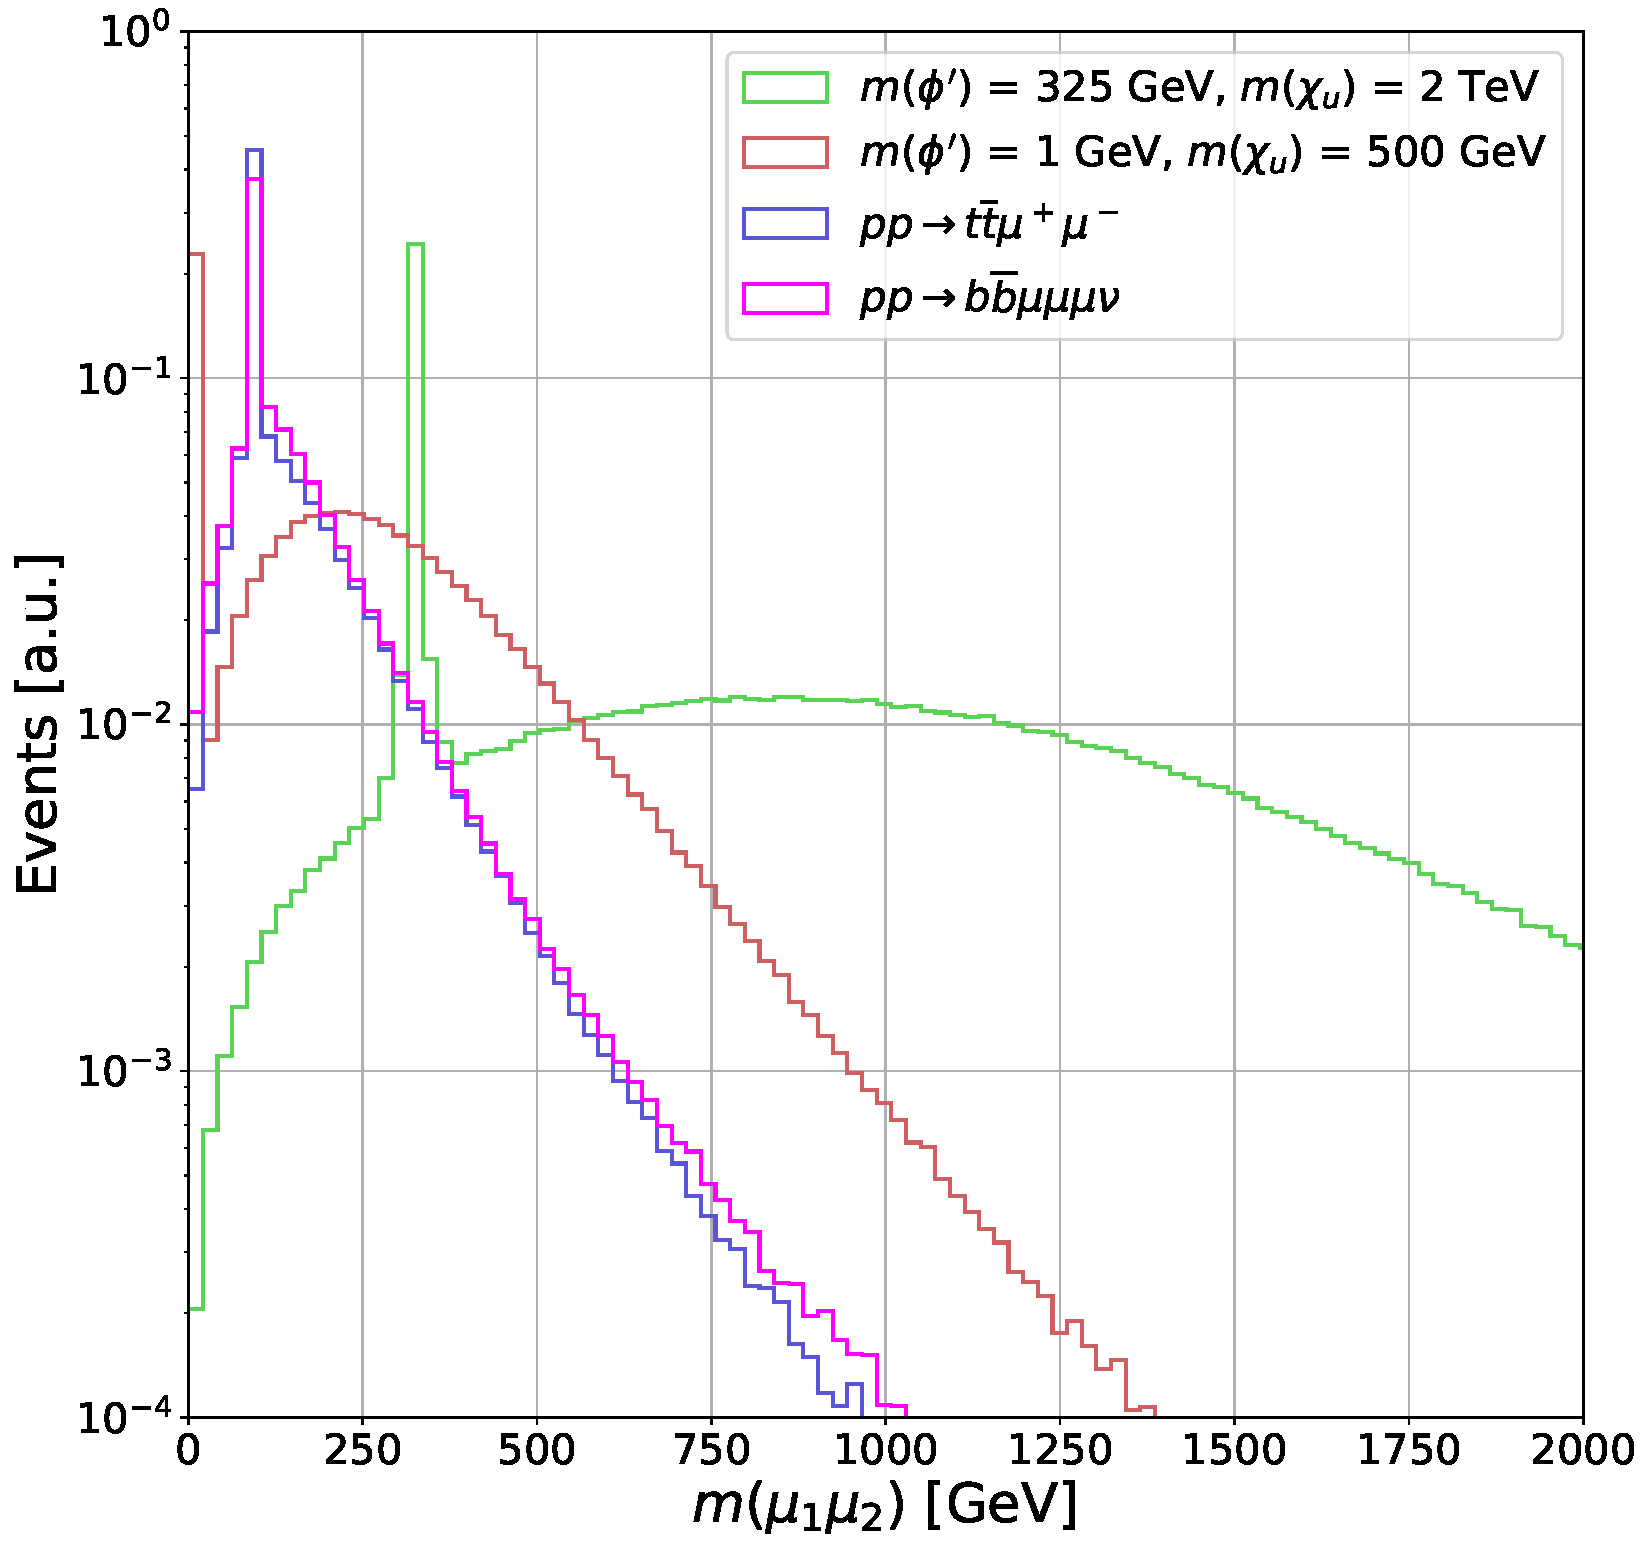
\includegraphics[width=.95\linewidth]{Images/M_mu_1_2.pdf}
\caption{Invariant mass distribution of the muon pair with the highest and second highest transverse momentum. The distributions are shown for the two main SM background processes and two signal benchmark points.\label{fig:_mu12}}
\end{figure}

We explore the performance of a diverse set of machine learning models, specifically three neural networks of differing architectures and a BDT algorithm. To ensure robust model assessment, we employed a standard 90-10 train-test split of the dataset, partitioning it into a 90\% portion for training and a 10\% portion for testing. This division allows us to gauge the generalization capabilities of our models on unseen data.  

The training and evaluation of the BDT were carried out in a high-performance computing environment. Specifically, an Nvidia A100 GPU was used. The canonical \texttt{PyTorch}~\parencite{paszke2019} deep learning framework was employed for configuring, training, and evaluating the neural networks. PyTorch is well-regarded for its flexibility and performance in deep learning applications.

For the BDT algorithm, we used hyperparameters $\eta=0.3$, $\gamma = 0$, and $\texttt{max\_depth} = 6$. The \texttt{XGBoost}~\parencite{chen_xgboost_2016} library was used for the implementation of the Boosted Decision Tree algorithm. It offers high efficiency, optimization, and interpretability, making it a suitable choice for this particular task. 

\begin{figure}
\centering
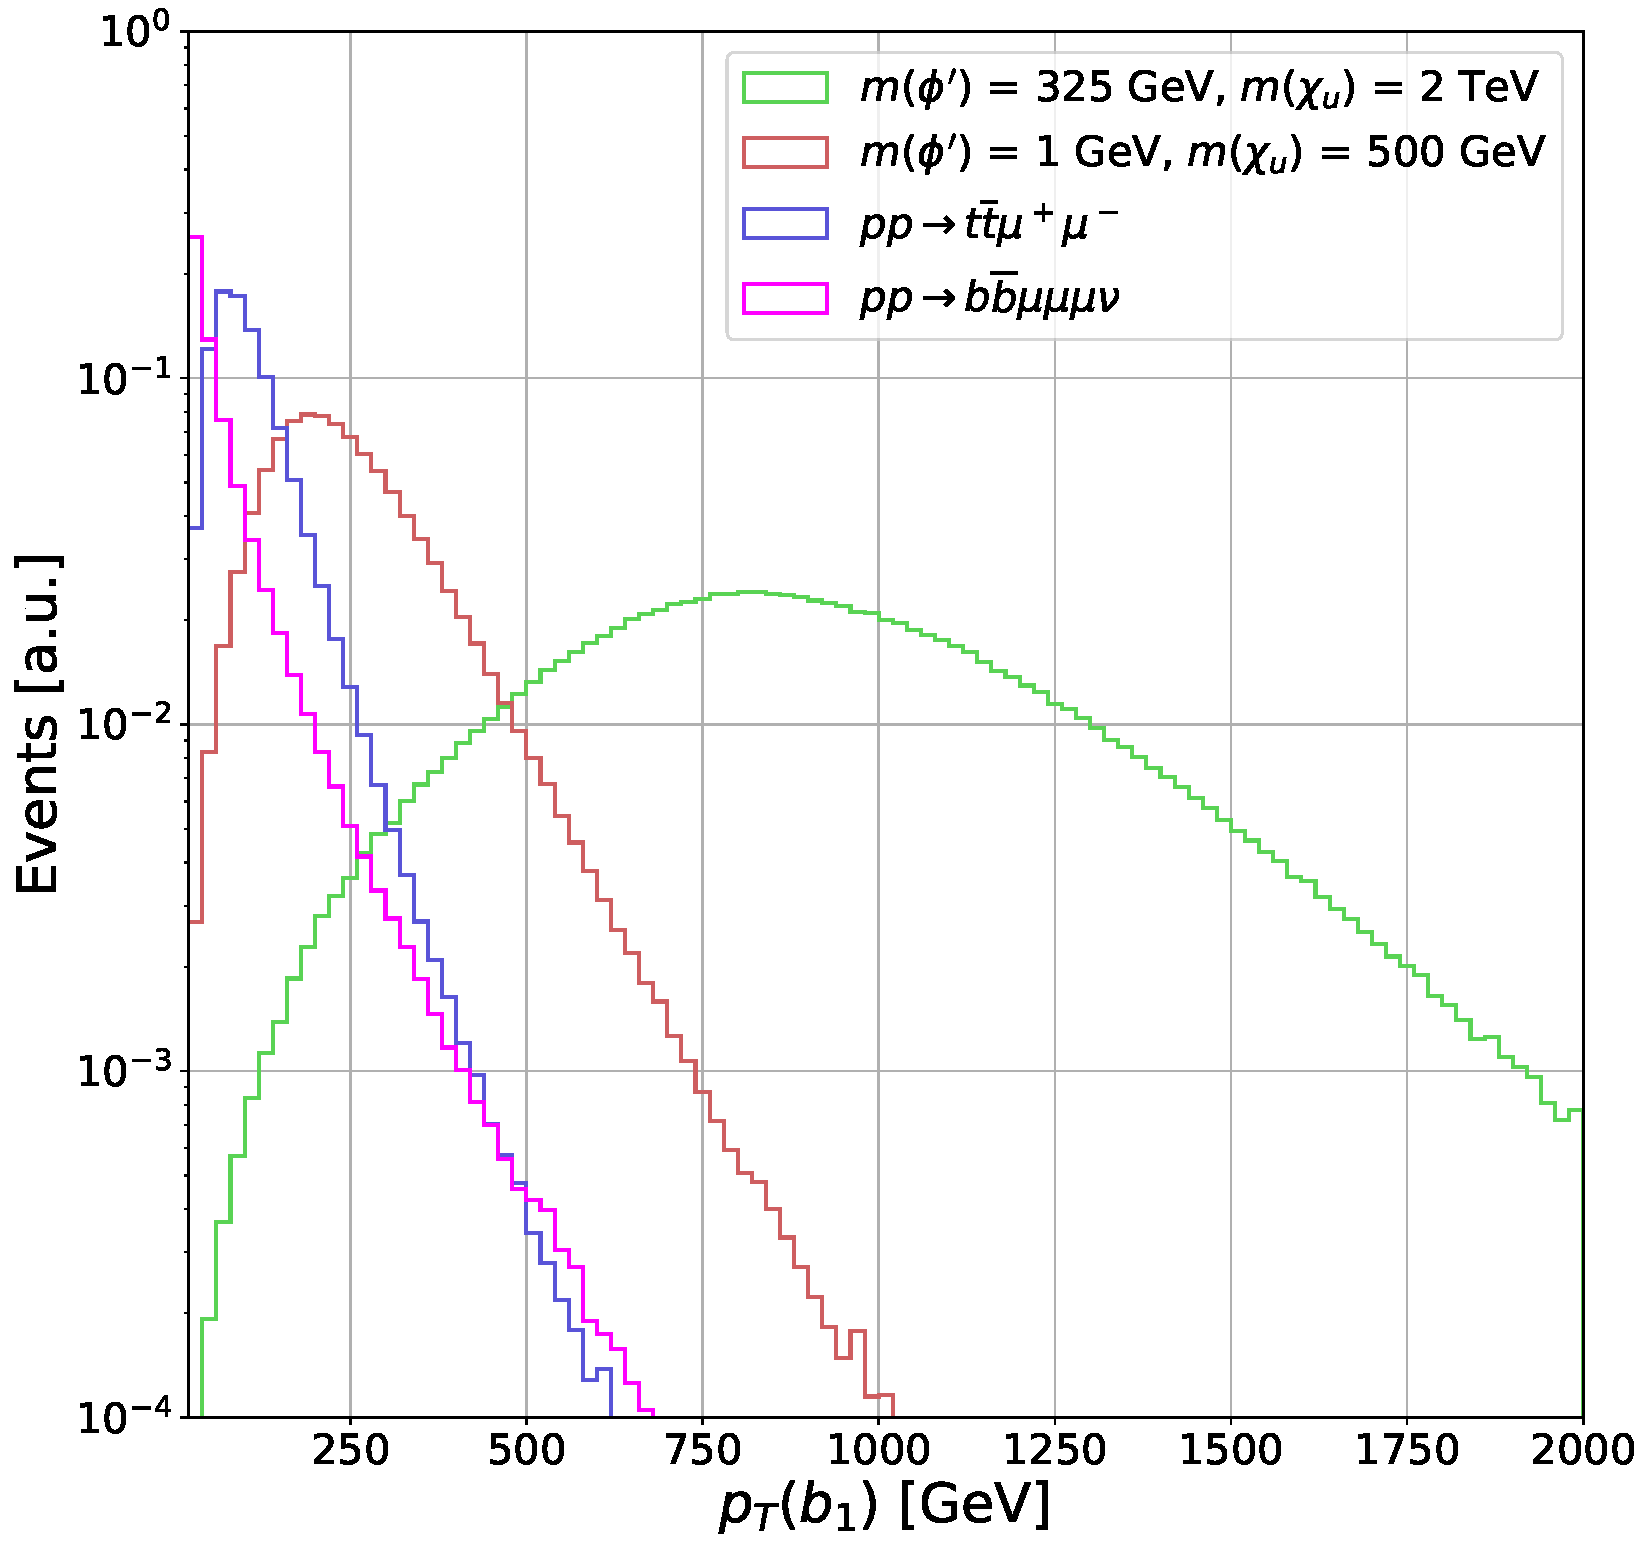
\includegraphics[width=.75\linewidth]{Images/PT_b1.pdf}
\caption{Transverse momentum distribution of the leading \textrm{b}-quark jet candidate. The distributions are shown for the two main SM background processes and two signal benchmark points.\label{fig:pTb1}}
\end{figure}

\begin{figure}
\centering
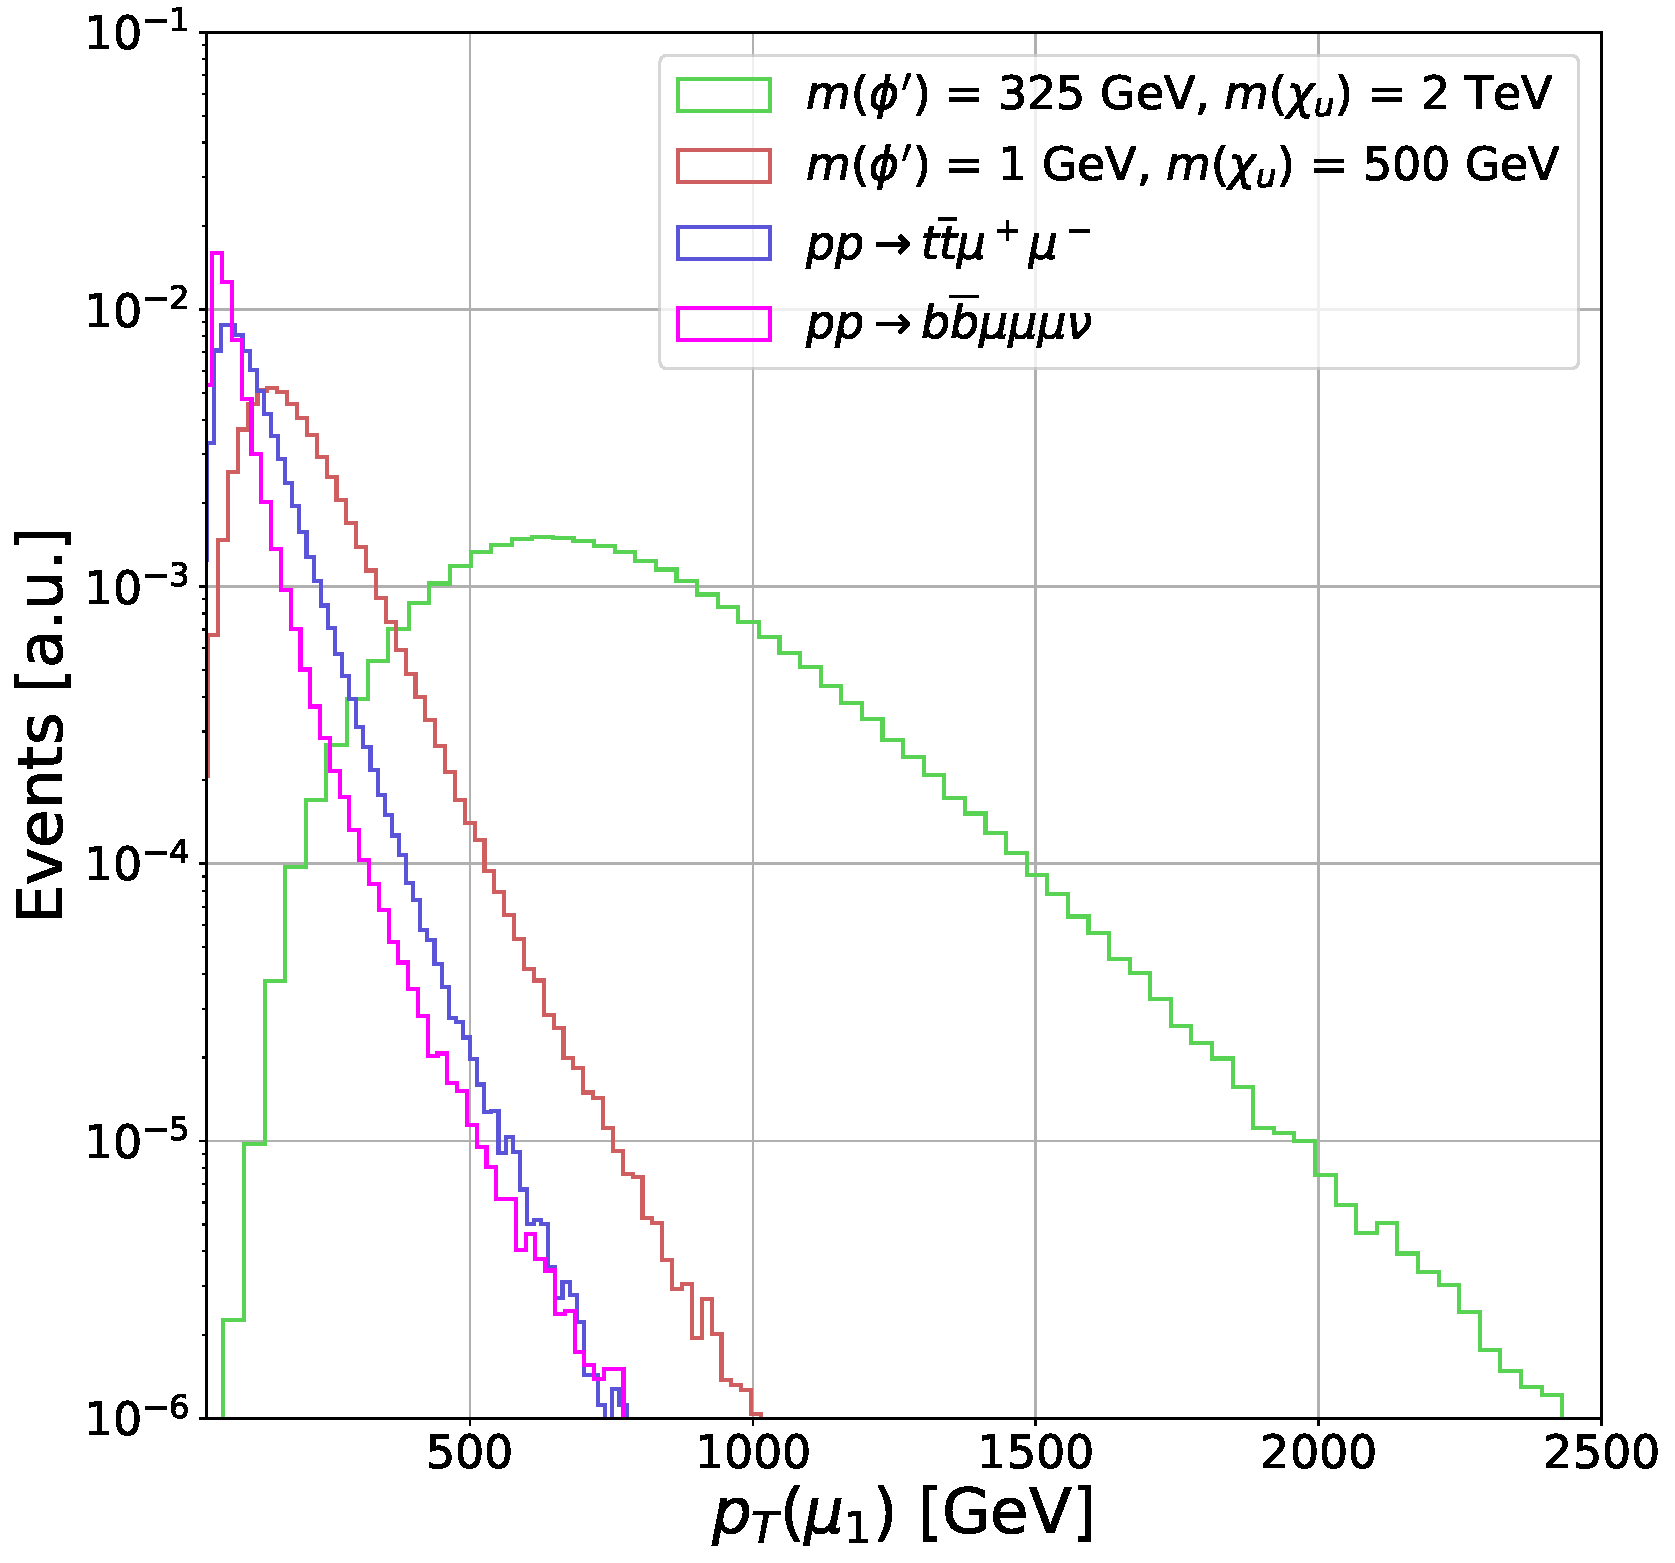
\includegraphics[width=.75\linewidth]{Images/PT_mu1_1.pdf}
\caption{Transverse momentum distribution of the leading muon candidate. The distributions are shown for the two main SM background processes and two signal benchmark points.\label{fig:pTmu1}}
\end{figure}

\begin{table}
    \centering
    \begin{tabular}{c  c  c}
    \hline
    { Model} & { Train/Test Acc. } & { Training Time} \\
    \hline
    \small
    BDT & N.A./0.9993  & 6s\\
    Neural Network 1 & 0.9999/0.9997 & 1h 58m \\
    Neural Network 2 & 0.9999/0.9998 & 2h 12m \\
    Neural Network 3 & 0.9999/0.9998 & 2h 32m\\
    \hline
    \end{tabular}
    \caption{Train/test results for the ML models.}\label{tab:ml_results}
    \centering
\end{table}

It is worth mentioning that we experimented with deep neural networks of various architectures. Although we found that they yield similar signal sensitivity to the BDT, the complex nature of the studies in this
work (particle objects considered, experimental constraints in a high luminosity LHC, etc.) motivates the use of a BDT over a deep neural network because of its usefulness, efficiency, and simplicity in understanding the machine learning output in addition to significantly shorter training times. Therefore, we perform our proceeding analysis using the BDT. The outcomes of our model training and evaluation are presented in Table 3. 
